\documentclass[12pt,a4paper]{article}

\usepackage[fleqn]{amsmath} % This package with the fleqn option aligns equations to the left
\setlength{\mathindent}{0pt} % Set indentation from the left margin

\usepackage{amssymb} % Required for math symbols
\usepackage{graphicx} % Required for inserting images
\usepackage{geometry}

\usepackage{subcaption}

\PassOptionsToPackage{hyphens}{url}\usepackage{hyperref}

\usepackage[backend=biber, style=authoryear, citestyle=authoryear]{biblatex}
\addbibresource{references.bib}

\geometry{a4paper, margin=1in}

{
\title{
    
\includegraphics[width=0.34\textwidth]{/Users/mlnick/documents/images/tsukuba-logo.png} \\
    \vspace{2mm}
    \textbf{Practical Development for IoT and Embedded Systems} \\
    \vspace{3mm}    
    Final Report on Team Project \\
    Virtual Display Interaction System
}

\author{Mamanchuk Mykola, SID.202420671}
\date{\today}
}

\usepackage{listings}
\usepackage{color}

\definecolor{codegreen}{rgb}{0,0.6,0}
\definecolor{codegray}{rgb}{0.5,0.5,0.5}
\definecolor{codepurple}{rgb}{0.58,0,0.82}
\definecolor{backcolour}{rgb}{0.99,0.99,0.99}

\lstdefinestyle{mystyle}{
    backgroundcolor=\color{backcolour},   
    commentstyle=\color{codegreen},
    keywordstyle=\color{magenta},
    numberstyle=\tiny\color{codegray},
    stringstyle=\color{codepurple},
    basicstyle=\ttfamily\footnotesize,
    breakatwhitespace=false,         
    breaklines=true,                 
    captionpos=b,                    
    keepspaces=true,                 
    numbers=left,                    
    numbersep=5pt,                  
    showspaces=false,                
    showstringspaces=false,
    showtabs=false,                  
    tabsize=2
}
\lstset{style=mystyle}

\begin{document}

\maketitle

\section{Introduction}

\subsection{Abstract}
In the world of technology, touchscreens have become ubiquitous, found in everything from smartphones to interactive kiosks. Traditional touchscreen technologies rely on expensive laser-based systems to detect touch, making them cost-prohibitive for many applications. 

\begin{figure}[!htp]
    \centering
%    \textbf{Your title}\par\medskip
    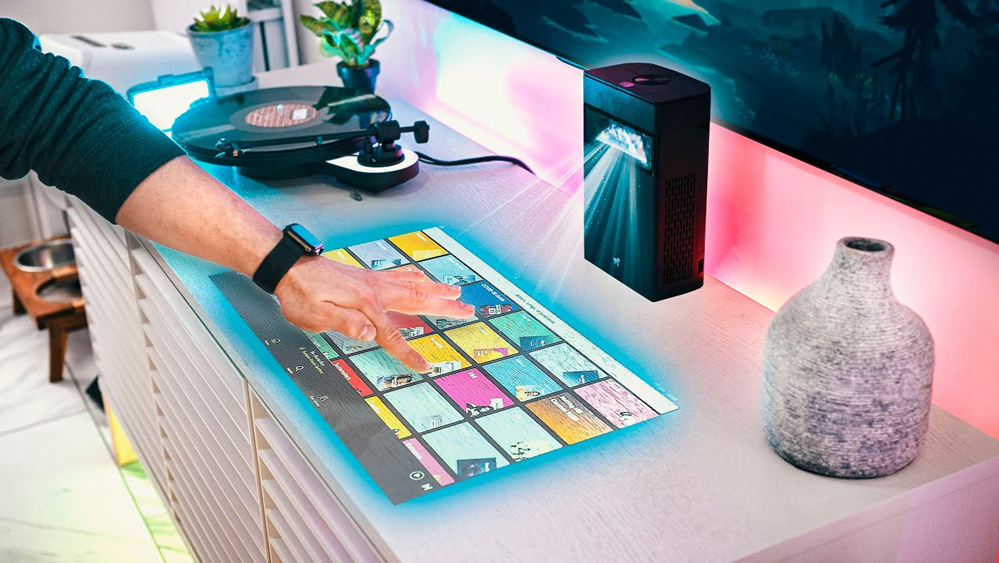
\includegraphics[scale=0.5]{../IoT Materials/article images/0-Expensive-lazer-technology.png}
    \caption{Contemporary lazer-based virtual screen technology is expensive}
\end{figure}

This project aims to develop a cost-effective solution by utilizing inexpensive distance sensors to simulate a touchscreen. This innovation can redefine user interaction, making touchless control accessible for a broader range of applications, including education, healthcare, and entertainment. \textbf{The article published on Design Spark} regarding the idea, development, implementations, and other essentials \textbf{can be reviewed following [1] in the reference section}.

\subsection{Objective}
The primary objective of this project is to create an interactive touchscreen system using low-cost distance sensors. By achieving this, the project seeks to provide a viable alternative to traditional touchscreen technologies, reducing costs while maintaining functionality and accuracy.



\section{Development Background}

\subsection{Motivation}
The motivation behind this project stems from the desire to create an affordable and accessible touchless interaction system. Traditional touchscreens, which rely on expensive laser technology, are cost-prohibitive for many users and applications. Our team aimed to explore the potential of using low-cost distance sensors to simulate a touchscreen, making the technology more accessible and cost-effective.

The project requirements specified the use of Raspberry Pi, which led us to consider various practical applications for this device. We focused on a frequent activity at home—cursor control. While there are commercial gadgets available that offer similar functionality, they are often expensive. Our goal was to develop a budget-friendly alternative that could inspire others to create similar solutions using different means, such as Bluetooth listeners. This project not only addresses a practical need but also provides an interesting research opportunity in the field of IoT and interactive systems.

\subsection{Initial Research}
Our initial research involved exploring the concept of trilateration, a method commonly used in navigation and positioning systems. Trilateration involves calculating the position of an object based on the known distances from three fixed points. We hypothesized that this method could be adapted to determine the position of a user's hand relative to the touchscreen.

\begin{figure}[!htp]
    \centering
    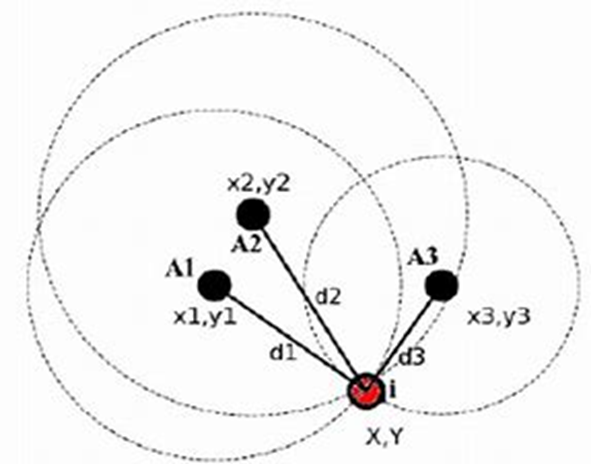
\includegraphics[scale=0.3]{../IoT Materials/article images/1-Trilateriation-diagram.png}
    \caption{Diagram illustrating the concept of trilateration}
\end{figure}

We found a relevant study on the Arduino Forum [2] that described the use of modified HC-SR04 sensors for triangulating the position of objects. This study provided valuable insights and a foundation for our project.

\subsection{Project Goals}
The primary goals of our project were:
\begin{itemize}
    \item To develop a cost-effective virtual touchscreen system using distance sensors.
    \item To explore the application of trilateration in interactive systems.
    \item To learn and apply IoT concepts and techniques in a practical project.
    \item To foster teamwork and collaboration among team members.
\end{itemize}

These goals were designed to address the identified need for an affordable touchless interaction system while providing a valuable learning experience for all team members. The project allowed us to work on a real-world problem, apply theoretical knowledge, and develop practical skills in IoT and interactive system design.

\begin{figure}[!htp]
    \centering
    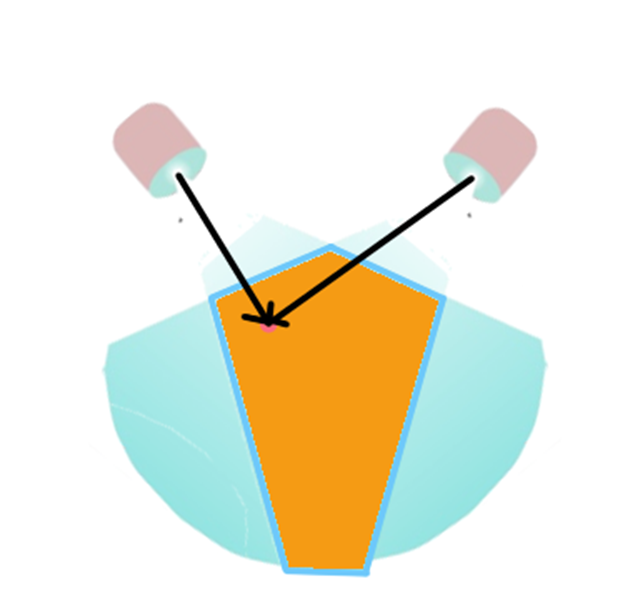
\includegraphics[scale=0.3]{../IoT Materials/article images/3-Concept-schematics.png}
    \caption{Concept schematics of the virtual touchscreen system}
\end{figure}

Through this project, we aimed to contribute to the field of IoT by developing a practical, innovative solution and to inspire others to explore similar low-cost technologies. Additionally, we gained insights into team dynamics, project management, and the importance of clear communication and collaboration in achieving project success.

\section{Design and Implementation}

\subsection{System Design}
The overall system architecture is designed to simulate a touchscreen using low-cost distance sensors. The system consists of a Raspberry Pi connected to two HC-SR04 ultrasonic sensors. These sensors measure the distance to the user's hand and use trilateration to determine its position. The design choices focused on cost-effectiveness and simplicity, making the system accessible for various applications.

\subsection{Hardware Components}
The following hardware components were used in the project:
\begin{itemize}
    \item \textbf{Raspberry Pi 4 Type B}: This small computer processes the data from the sensors and controls the entire system.
    \item \textbf{Breadboards}: Used for prototyping and connecting components.
    \item \textbf{HC-SR04 Ultrasonic Distance Sensors}: Inexpensive and high-precision distance measurement sensors. The project uses two sensor blocks.
\end{itemize}

\begin{figure}[!htp]
    \centering
    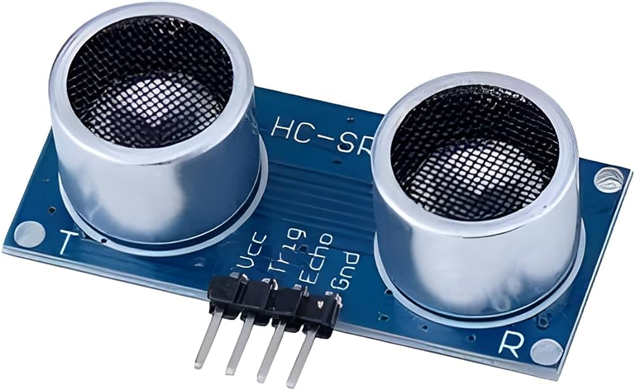
\includegraphics[scale=0.3]{../IoT Materials/article images/6-Infrared-sensor.png}
    \caption{One of the HC-SR04 sensors used in the project. Each block contains two sensors.}
\end{figure}

\begin{figure}[!htp]
    \centering
    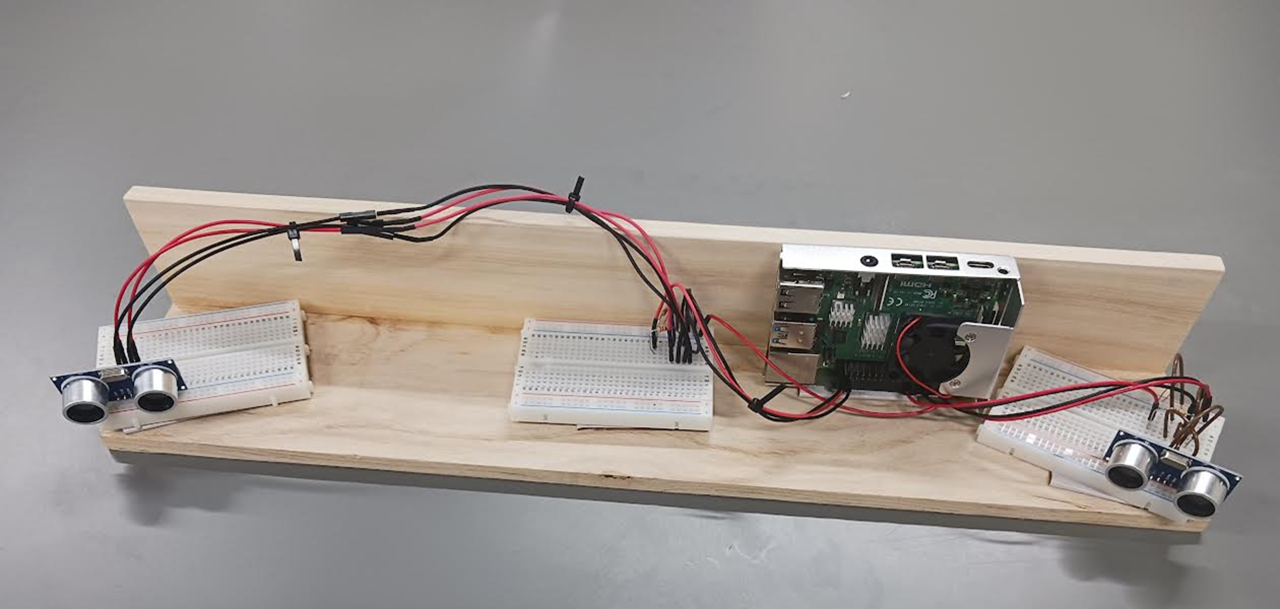
\includegraphics[scale=0.3]{../IoT Materials/article images/7-Test-stand.png}
    \caption{The setup and configuration of the test stand.}
\end{figure}

The test stand combines the above components with two sensor blocks facing each other at an angle of approximately 30 degrees to create a convenient intersection area. All components are connected to a central breadboard. The Raspberry Pi is powered from a socket, and data is recorded and updated every 0.5 seconds using the latest version of Python.

\subsection{Software Implementation}
The software component of this project is crucial for processing the sensor data and simulating the touchscreen. The system is primarily written in Python, utilizing several libraries for handling sensor input, data processing, and graphical display.

All source code files refered in this subsection can be reviewed following the Github link for project's repository [3].

The main components of the software are:

\begin{itemize}
    \item \textbf{Sensor Data Processing:} This involves reading data from the HC-SR04 sensors using the Raspberry Pi's GPIO pins. The data is processed to calculate the distances between the sensors and the hand. The relevant functions and logic for this are found in the \texttt{main.py} and \texttt{touchscreen.py} files.
    \item \textbf{Trilateration Algorithm:} The trilateration algorithm is implemented to determine the position of the hand based on the distances calculated from the sensors. This logic is primarily located in the \texttt{trilateration.py} file.
    \item \textbf{Graphical Interface:} The graphical interface displays the simulated touchscreen and responds to the hand movements detected by the sensors. The interface is developed using Kivy, a Python framework for developing multitouch applications. The relevant code for this is in the \texttt{rawdrawer.py} file.
    \item \textbf{Server Communication:} The system includes a server component that allows remote control and monitoring of the touchscreen simulation. This is handled in the \texttt{server.py} file.
\end{itemize}

Below is a brief explanation of some key functions:
\begin{itemize}
    \item \texttt{main.py} handles the initialization and coordination of the various components.
    \item \texttt{touchscreen.py} contains functions for reading sensor data and performing initial processing.
    \item \texttt{trilateration.py} includes the trilateration algorithm to calculate the hand's position.
    \item \texttt{rawdrawer.py} manages the graphical display and user interface.
    \item \texttt{server.py} handles network communication for remote control.
\end{itemize}

The detailed code implementation can be found in the Appendix A.

\subsection{Trilateration Theory}
Trilateration is a method of determining the position of a point by measuring distances to it from known points. Unlike triangulation, which uses angles, trilateration relies solely on distance measurements.

In this project, trilateration is used to determine the position of the hand in a 2D plane using three HC-SR04 ultrasonic sensors. The basic principle involves solving for the intersection of three circles, each centered at a sensor with a radius equal to the measured distance to the hand.

The equations for trilateration in a 2D space are as follows:

\[
\begin{cases}
(x - x_1)^2 + (y - y_1)^2 = d_1^2 \\
(x - x_2)^2 + (y - y_2)^2 = d_2^2 \\
(x - x_3)^2 + (y - y_3)^2 = d_3^2
\end{cases}
\]

Where \((x_1, y_1)\), \((x_2, y_2)\), and \((x_3, y_3)\) are the coordinates of the sensors, and \(d_1\), \(d_2\), and \(d_3\) are the measured distances from each sensor to the hand.

To solve these equations, the differences between pairs of equations are taken to eliminate the quadratic terms, leading to a system of linear equations that can be solved using standard algebraic methods.

In the context of our implementation:
\begin{itemize}
    \item The function \texttt{calculate\_position()} in \texttt{trilateration.py} performs the trilateration calculation.
    \item The sensors' positions and distances are read and processed in \texttt{touchscreen.py}.
    \item The graphical representation of the calculated position is handled by \texttt{rawdrawer.py}.
\end{itemize}

Trilateration is a well-established method in fields such as surveying and navigation. The mathematical foundations and practical applications of trilateration are detailed in the Appendix, including the derivation of the equations and the solution process.

\begin{figure}[!htp]
    \centering
    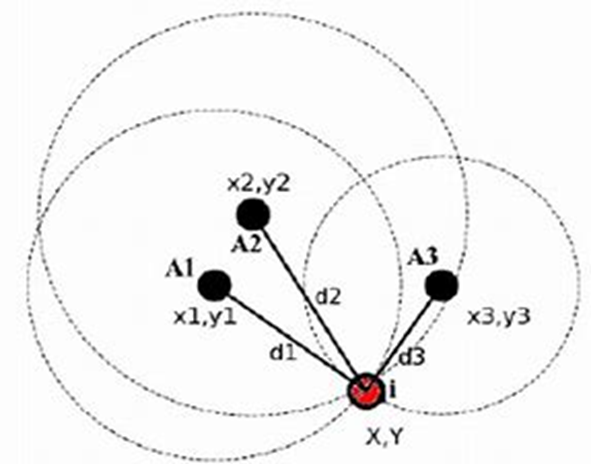
\includegraphics[scale=0.4]{../IoT Materials/article images/1-Trilateriation-diagram.png}
    \caption{Diagram showing the trilateration concept used in the project.}
\end{figure}

The detailed derivation and explanation of the trilateration algorithm can be found in the provided reference on Wikipedia [4].

This concludes the explanation of the trilateration theory and software implementation for our project. The code and more detailed explanations can be found in the Appendix.

\subsection{Calibration and Configuration}
The calibration process for the sensors involves defining the effective area where the virtual touchscreen operates. This area corresponds to the intersection sector of the rays fired by the sensors.

\begin{figure}[!htp]
    \centering
    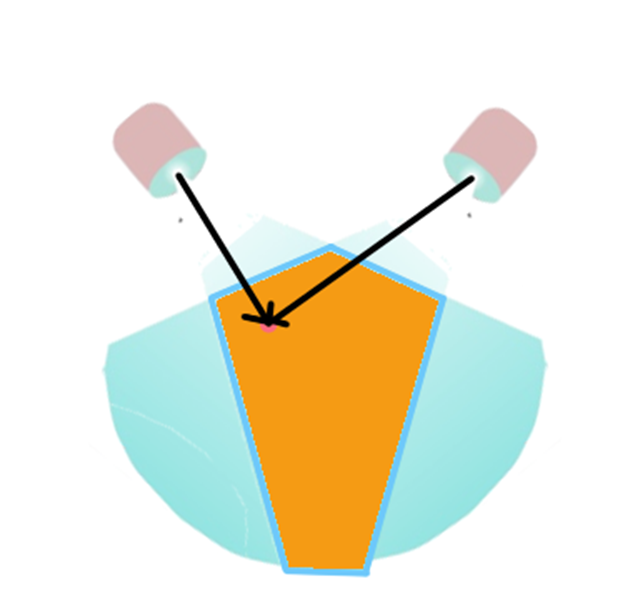
\includegraphics[scale=0.3]{../IoT Materials/article images/3-Concept-schematics.png}
    \caption{Conceptual schematics of the system.}
\end{figure}

Once the effective area is defined, the goal is to define the rectangular area of the virtual touchscreen, which corresponds to the area read to move the cursor on the screen of interest.

\begin{figure}[!htp]
    \centering
    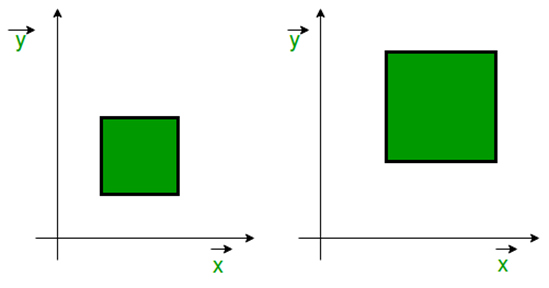
\includegraphics[scale=0.3]{../IoT Materials/article images/4-Calibration-diagram.png}
    \caption{Calibration diagram.}
\end{figure}

The system connects the device of interest (smartphone or PC with a screen) via UDP to the Raspberry Pi stand, which switches into the listening node with its sensors.

\begin{figure}[!htp]
    \centering
    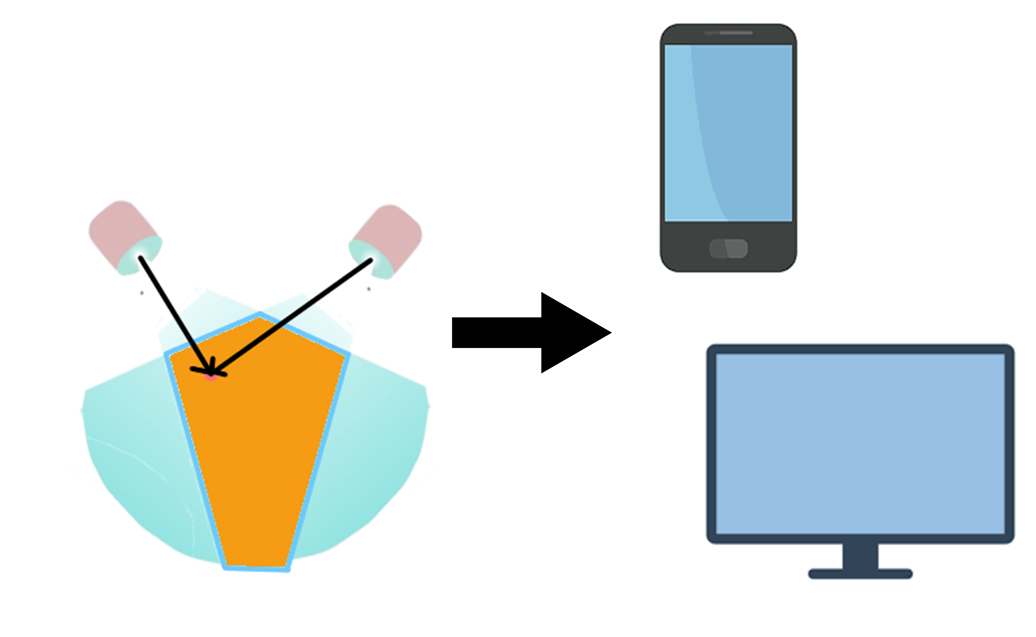
\includegraphics[scale=0.3]{../IoT Materials/article images/5-Concept-transition-device-relation.png}
    \caption{Device connection and data flow.}
\end{figure}

% APPLICATION SHOWCASE
\section{Application Showcase}
\subsection{Initial Usage Instructions}
This section provides step-by-step instructions on how to use the application. The video demonstration can be accessed following the link [5] in the reference list.

First and foremost, a device has to be connected to the same network as the Raspberry PI. Then, after the application loaded, we are presented with a user GUI. Control interface is simple and consists of 5 buttons. At this stage, proceed with pressing "Connect" and wait until the popup with a cursor appears. The procedure of connection and calibration is illustrated below on the Figure 10.

\begin{figure}[htbp]
    \centering
    \begin{subfigure}{0.45\textwidth}
        \centering
        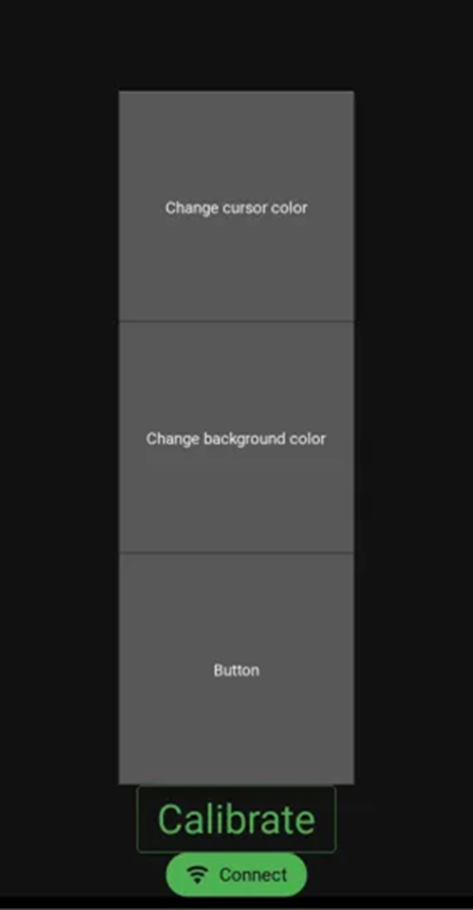
\includegraphics[scale=0.4]{../IoT Materials/article images/8-Screen-showcase-startup.png}
        \vspace{8mm}
        \caption{Application startup screen showcasing the initial stage and buttons: Change cursor color, Change background color, Button, Calibrate, and Connect.}
        % \vspace{2em} % Add vertical space to align the captions
    \end{subfigure}
    \hfill
    \begin{subfigure}{0.45\textwidth}
        \centering
        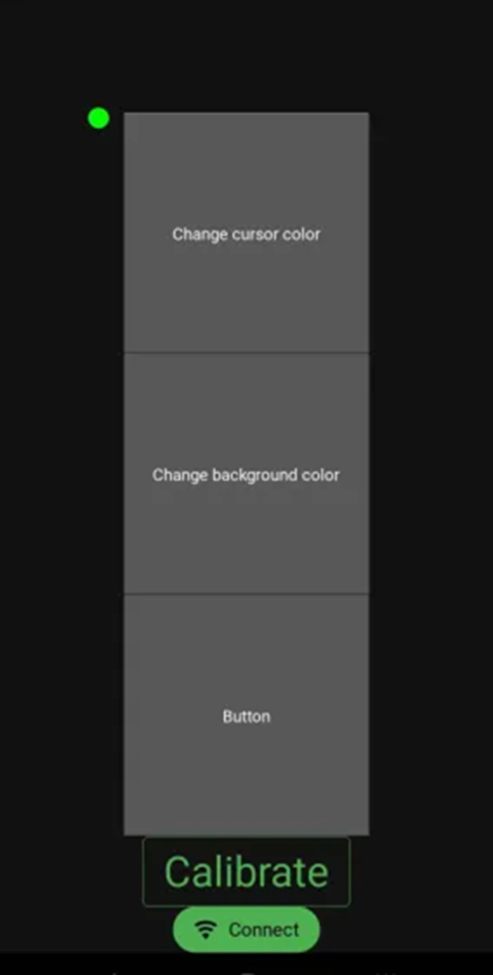
\includegraphics[scale=0.4]{../IoT Materials/article images/9-Screen-showcase-with-pointer-after-connection.png}
        \caption{After connecting the device to the same network as the Raspberry Pi and pressing the connect button, the established connection message appears, and the cursor is displayed on the screen.}
    \end{subfigure}
    \caption{Application Startup and Connection}
\end{figure}

\begin{figure}[htbp]
    \centering
    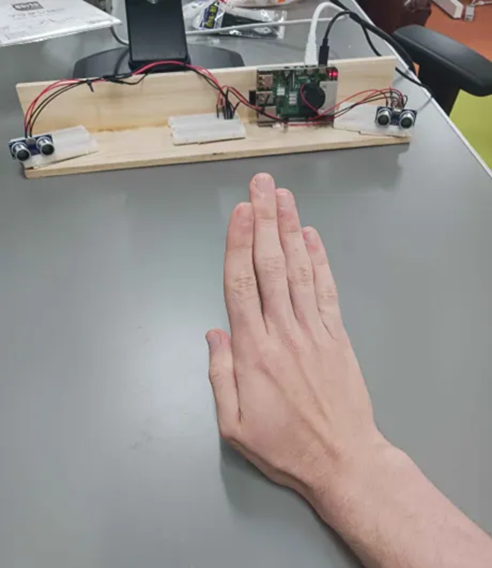
\includegraphics[scale=0.7]{../IoT Materials/article images/10-Using-hand-for-calibration.png}
    \caption{Quick practical check}
\end{figure}

Here, simply try moving a hand in front of the sensors as shown on the Figure 11. Once a cursor movement on the screen is detected, proceed with calibration.

\subsection{Calibration Process}

\begin{figure}[htbp]
    \centering
    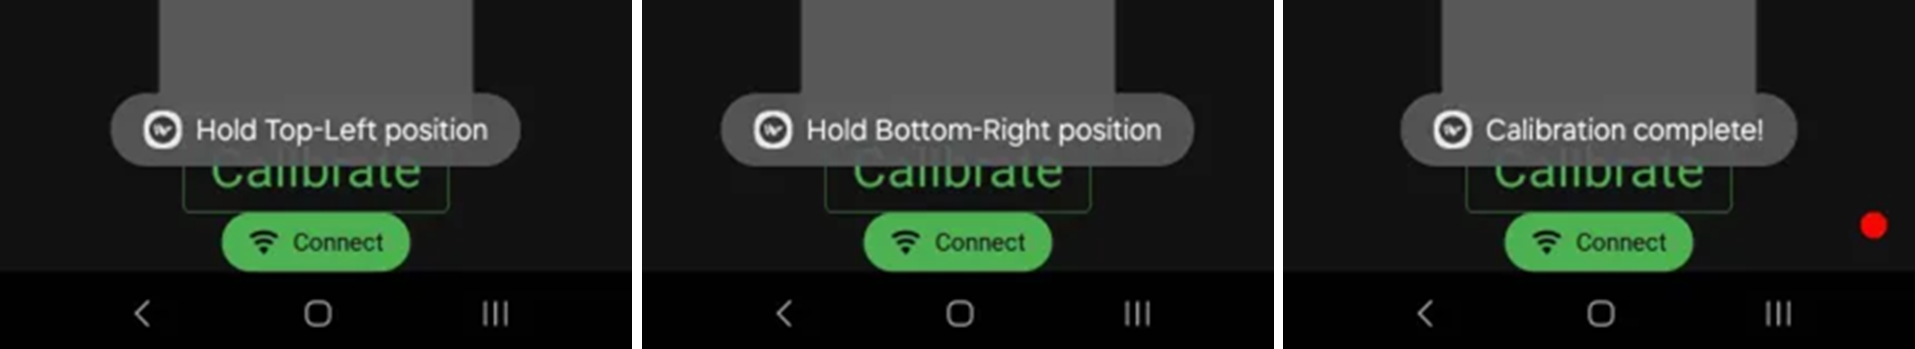
\includegraphics[scale=0.4]{../IoT Materials/article images/11-Screen-showcase-calibration-procedure.png}
    \caption{Calibration procedure showcase}
\end{figure}

\textbf{Calibration steps}
\begin{itemize}
    \item Define the rectangle within the effective area of intersecting rays.
    \item Tap the calibrate button and move your hand to the top-left position of the defined mapping space. Hold your hand until calibration is completed.
    \item Move and hold your hand to the bottom-right corner of the space until the calibration completion message is displayed.
\end{itemize}

After finishing the listed process, you can use the defined effective area as a virtual display to move the cursor around the screen, where the position of your hand in this area maps to the desired spot on the screen. Holding the hand in position triggers a click.

\begin{figure}[htbp]
    \centering
    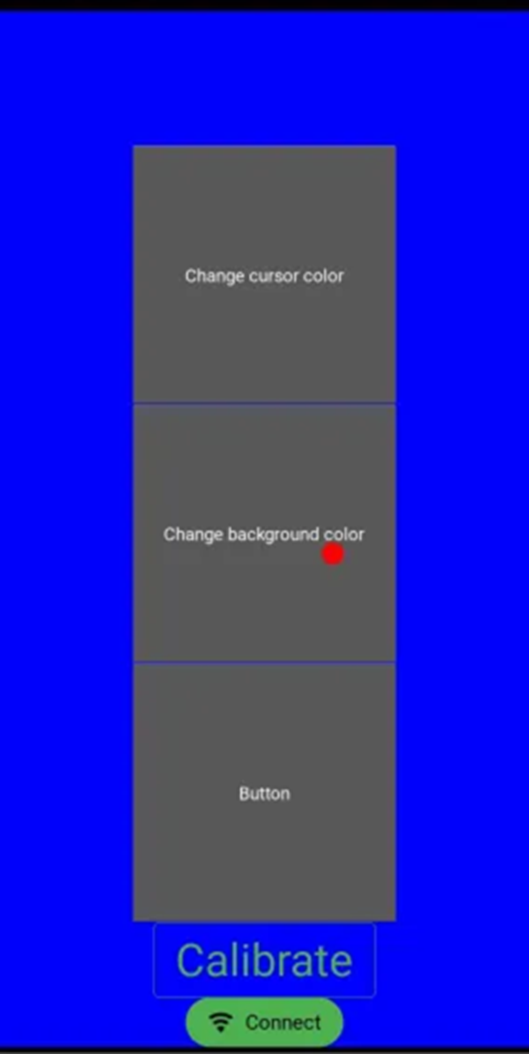
\includegraphics[scale=0.4]{../IoT Materials/article images/12-Screen-showcase-click.png}
    \caption{Click showcase: changing background color of the application}
\end{figure}

\section{Improvements and Potential Integrations}

While the idea of using infrared sensors in such system is perspective, we found many constaints which are related to the quality of used components and particular design approach.

Below are listed some ideas and observations, which are essential to consider upon further improvement of the concept:

\begin{itemize}
    \item For infrared emitters, the calculation is most precise if the pointing object (e.g., hand) is round. This is crucial during calibration, as a precisely calibrated area results in more accurate mapping.
    \item The current implementation is limited by the design and characteristics of infrared radiation, using only two infrared sensor blocks. Using more sensors could make position calculations more accurate and reduce delay related to averaging calculations.
    \item Incorporating ML algorithms to preprocess data and reduce noise could improve system performance, especially when the pointing object is not perfectly round.
\end{itemize}

\begin{figure}[htbp]
    \centering
    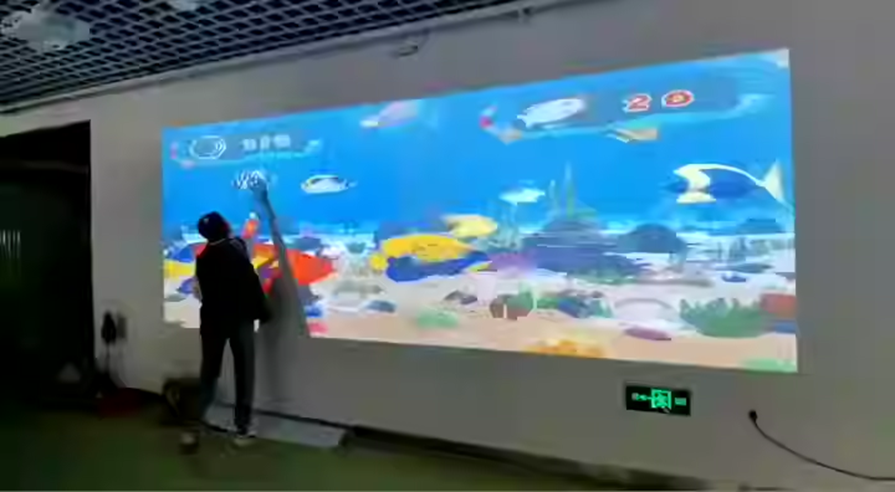
\includegraphics[scale=0.6]{../IoT Materials/article images/14-Additional-distracting-3.png}
    \caption{Projecting systems with touchscreen capability can become more affordable}
\end{figure}

To conclude, this technology holds potential for applications in education, healthcare, and entertainment, with future improvements enhancing its interactive capabilities.

\section{Personal Contribution}
\subsection{My Role in the Project}

I find it fascinating that before the team project assignment was introduced, a special lecture on team building was included in the course of Practical Development of IoT and Embedded Systems. (For additional information, you can refer to the file with the report on team building - there is some information on my anticipations which I to some extent managed to execute in the process of development).

\subsubsection{Responsibilities and Tasks}
My responsibilities within the project development team included activities related to project testing, development assistance, GitHub branch creation and management, considerations upon presentations, development, creation, and publication of the article in Japanese related to the project, and general assistance with making the final report.

During the development process, I have discussed potential directions with my team on how the project would be better designed and presented. I provided testing assistance and ideas for debugging and error fixes and improvements. I also tested the project on my machine to check cross-platform compatibility.

While the main developers of the project were my teammates due to me being abroad during the development weeks, I have been engaged in planning activities and team building while ensuring that the development goes according to the anticipated plan.

\subsubsection{Specific Contributions}
Specifically, I contributed to tuning the calculation procedure and recorded parameters so that the behavior of the system becomes smoother. I have encountered several issues related to the compatibility and behavior of the application. Those have been fixed upon considering with the whole team.

\subsection{Challenges Faced}
\subsubsection{Technical Challenges}
Technical challenges included the initial setup of the system, choice of data exchange protocols, binding of the devices with a Raspberry Pi node, and assembling of the stand. The most important faced was with the choice of sensors and the design in general. Since infrared sensors are used, they are highly sensitive to imperfectly round objects which produce much noise. At the same time, there are only two utilized sensor blocks - two sensors in each block which makes these two sensors in one block be closely located. This resulted in the situation with interference of the light - and the data became noisy which was unusable for the system in the current software implementation. Therefore, a conclusion for averaging the recorded data for an extended period was reached - which led to constraints but fixed the appeared issue.

\subsubsection{Resolution Strategies}
To overcome technical challenges, the team was engaged in regular discussions and read many articles related to similar calculations and system integration protocols.

\subsubsection{Project Management Challenges}
Since there practically were two weeks on the app development, team collaboration and time management were key strategies to develop a successful project ready for a showcase in the class and further publication of results. Regardless of the time difference between Japan and Europe, we were engaged in few calls to discuss further development strategies and deadlines.

\section{Insights and Learnings}
\subsection{Key Takeaways}
\subsubsection{Insights}
From this project, definitely the biggest thing I have learned is related to team building and teamwork. Since I was abroad, I understood that it is extremely difficult to find time for team calls. I also learned that your engagement directly influences the motivation of the entire team, therefore you can achieve exceptional results.

\subsubsection{Technical Learnings}
Since the start of the project, I have learned many new things related to the concepts used in the project, used technologies, theoretical details about the process of trilateration, and much more related to technical implementations of Raspberry Pi and embedded systems using breadboards and various components.

\subsubsection{Project Management Learnings}
Reflecting on the project management skills developed during the project, I realized the importance of proper planning, regular communication, and the use of tools such as GitHub for version control and collaboration.

\subsubsection{Team Collaboration}
Teamwork and collaboration were critical to the success of this project. Strategies that worked well included regular updates, clear task assignments, and leveraging each team member's strengths.

\subsection{Feedback and Reflection}
\subsubsection{Constructive Feedback}
I find the course well-designed, in particular, the resources and classes are conducted with assisting professors who offer help in any misunderstandings. I find the materials very detailed and kept up to date with the latest contributions and updates in API and programming languages versions. This way I elevated my proficiency using many concepts and development methodologies. I have worked in a team, where it was essential to understand how team building works, and how parallel development undergoes. I have also learned that project management can be a crucial process to follow even for a small-scale application and local enterprise teams. I have been engaged in the development process while contributing the best I could in my particular situation. I have learned that both personal initiative and collective decisions are integral parts of a successful development process. I hope to utilize this knowledge in my future projects while being more proactive in terms of direct development engagement and other project planning and promotion-related activities.

% \textbf{University of Tsukuba, Embedded Systems Development, 2024}



\section*{References}
\begin{enumerate}
    \item \textbf{Mamanchuk N. Design Sparks Community}, Published Article - Virtual touch screen Virtual touch technology with distance sensor. Available online: \url{https://www.rs-online.com/designspark/distance-sensor-virtual-touchscreen-jp} [Published: 2024-07-04]
    \item \textbf{Arduino Forum Library}, Online Forum - Using 3 modified hc-sr04 to triangulate the position of one or more objects, Sep2021. Available online: \url{https://forum.arduino.cc/t/using-3-modified-hc-sr04-to-triangulate-the-position-of-one-or-more-objects/902767} [Accessed: 2024-07-04]
    \item \textbf{Fernando Santos L., Sasaki N., Mamanchuk N. Project Development Team}, Github Repository - Virtual Display Interaction System, Jun2024. Available online: \url{https://github.com/RIFLE/iot-team-project} [Last Update: 2024-07-03]
    \item \textbf{Wikibedia - Free Encyclopedia}, Online Article - Trilateration. Available online: \url{https://en.wikipedia.org/wiki/Trilateration} [Accessed: 2024-07-04]
    \item \textbf{Fernando Santos L., Youtube}, Video Demonstration - Virtual Display Interaction System using Infrared Sensors. Available online: \url{https://www.youtube.com/watch?v=-euN-f_y6p8} [Accessed: 2024-07-05]
    % \item \textbf{Company}, Name of Work, year. Available online: \url{https://...} [Accessed: yyyy-mm-dd]
    \item \textbf{Mamanchuk N. University of Tsukuba}, Github, \today. Available online: \url{https://github.com/RIFLE}
\end{enumerate}

% \begin{center} 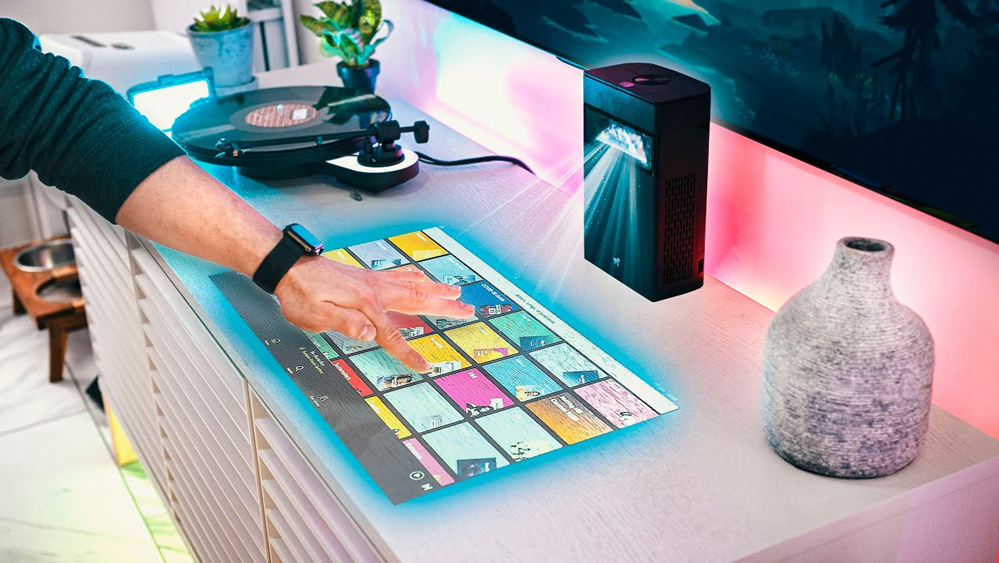
\includegraphics[width=0.34\textwidth]{../IoT Materials/article images/0-Expensive-lazer-technology.png}\end{center}

% \setlength{\fboxsep}{0pt} % Removes padding around the image
% \setlength{\fboxrule}{0.5pt} % Sets the thickness of the border

\newpage
\section*{Appendix A: Implementing Trilateration in Python}
%\begin{lstlisting}[language=Python, caption=Trilateration Code]
In the next listing, we show the implementation of the trilateration technique.

\begin{lstlisting}[language=Python]
    import numpy
    
    P1 = [0,0] #upper position
    P2 = [-10,10] #anyway position
    P3 = [10,10] #anyway position
    
    def trilateration(P1, P2, P3, r1, r2, r3):
        #r1,r2,r3 is the distance of staff and sensor
        p1 = numpy.array([0, 0])
        p2 = numpy.array([P2[0] - P1[0], P2[1] - P1[1]])
        p3 = numpy.array([P3[0] - P1[0], P3[1] - P1[1]])
        v1 = p2 - p1
        v2 = p3 - p1
        Xn = (v1)/numpy.linalg.norm(v1)
        tmp = numpy.cross(v1, v2)
        Zn = (tmp)/numpy.linalg.norm(tmp)
        Yn = numpy.cross(Xn, Zn)
        i = numpy.dot(Xn, v2)
        d = numpy.dot(Xn, v1)
        j = numpy.dot(Yn, v2)
        X = ((r1**2)-(r2**2)+(d**2))/(2*d)
        Y = (((r1**2)-(r3**2)+(i**2)+(j**2))/(2*j))-((i/j)*(X))
        Z1 = numpy.sqrt(max(0, r1**2-X**2-Y**2))
        Z2 = -Z2
        K1 = P1 + X * Xn + Y * Yn + Z1 * Zn
        K2 = P1 + X * Xn + Y * Yn + Z2 * Zn
        return K1,K2
\end{lstlisting}

\end{document}
